\subsection{Mini-Batch Gradient Descent}
We saw how vectorization allows us to perform forward and back propagation easily on $m$ training examples. 

$$
X_{(n_x, m)} = \begin{bmatrix}
    \vline &  & \vline\\
    x\idx{1} & \dots & x\idx{m}\\
    \vline &  & \vline
\end{bmatrix}
$$
$$
Y_{(1, m)} = 
\begin{bmatrix}
    y\idx{1} & \dots & y\idx{m}
\end{bmatrix} 
$$

What if $m=5000000$? We split our training set into mini batches of, say $1000$ training samples.
$$
X\ Batches: X\batch{1}, \dots, X\batch{5000}
$$ 
$$
Y\ Batches: Y\batch{1}, \dots, Y\batch{5000}
$$

\begin{itemize}
    \item for $t=1\dots5000$ do:
    \begin{itemize}
        \item[-] Forward Prop on $X\batch{t}$
        \begin{itemize}
            \item[] $Z\lay{1} = W\lay{1}X\batch{t}+b\lay{1}$
            \item[] $A\lay{1} = g\lay{1}(Z\lay{1})$ 
            \item[] $\dots$
            \item[] $Z\lay{L} = W\lay{L}A\lay{L-1}+b\lay{L}$
            \item[] $A\lay{L} = g\lay{L}(Z\lay{L})$ 
        \end{itemize} 
        \item[-] Compute Cost: $J\batch{t}=\frac{1}{1000}\sum{\dots} + \dots$
        \item[-] Back Prop to compute gradients with respect to $J\batch{t}$. 
        \item[-] Update parameters.   
    \end{itemize}
\end{itemize}

\subsection{Understanding Mini-Batch Gradient Descent}

\begin{figure}[H]
    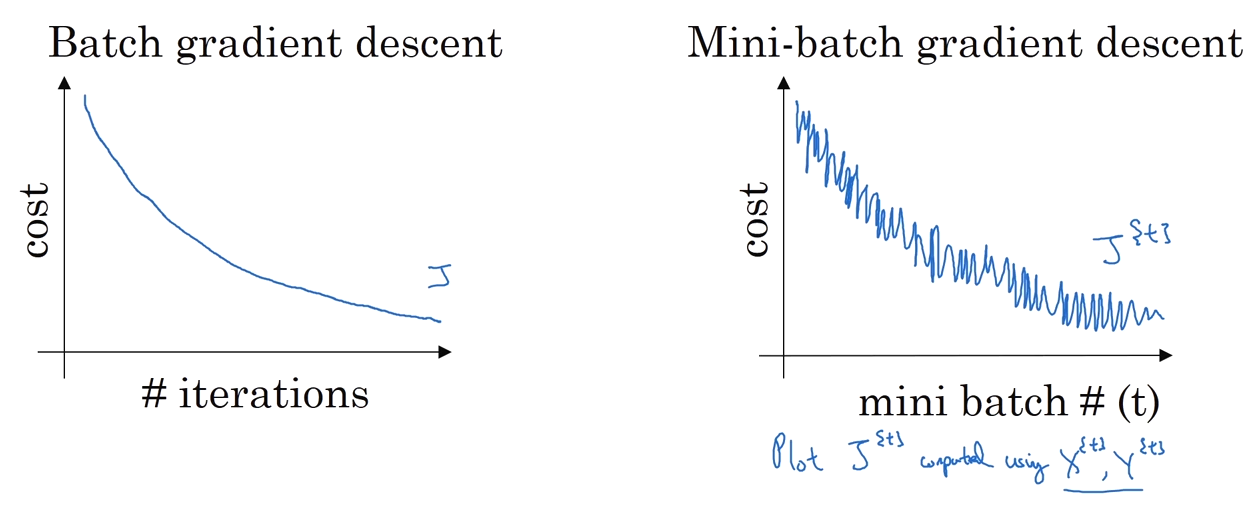
\includegraphics[scale=0.35]{images/minibatch.png}
    \centering
\end{figure}

\begin{itemize}
    \item If mini-batch size equals $m$: Batch Gradient Descent (Blue)
    \item If mini-batch size equals $1$: Stochastic Gradient Descent (Purple)
\end{itemize}

\begin{figure}[H]
    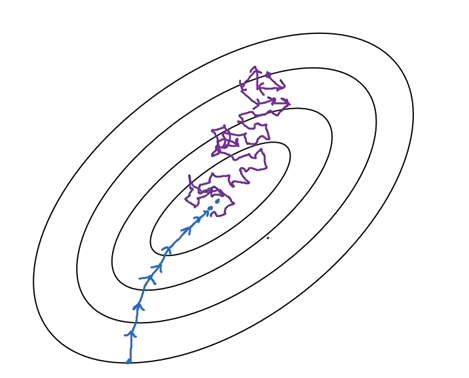
\includegraphics[scale=0.35]{images/stochastic.png}
    \centering
\end{figure}

\textbf{Batch Gradient Descent:} Too long per epoch.

\textbf{Stochastic Gradient Descent:} Losing the speed-up of vectorization. 

\textbf{Somewhere in Between:} Take advantage of the speed-up of vectorization + Make progress without needing to wait. Typical mini-batch sizes are $64, 128, 256, 512$. Make sure your mini-batches fit in CPU/GPU memory. 

